% first section should be classic supervised auto-encoder and maybe paris auto-encoder. then the next section can be dan stowells thing, and then finally the curro-net.
In the following sections, we detail all considered shallow network architectures. Note that these network architectures can easily be extended to deep networks by adding corresponding encode and decode layers before and after the latent representation, respectively. These networks can be trained using the various inputs detailed in Chapter 3. However, for the purposes of presenting first results, we consider single FFT frames only to compare networks. %In other words, we take overlapping frames of an audio signal $y[n]$ and pass their magnitude spectrum values $Y[k]$ into our network. The signal estimate $\hat{x}[n]$ is computed by taking the IFFT and using overlap-add reconstruction by combining the magnitude spectrum estimates with the original noisy phase:

% \begin{equation}
% \hat{X_i}[k] =
% \end{equation}

\subsection{Supervised Autoencoder}

We adopt the shallow supervised autoencoder from \cite{liu2014experiments}. Used for supervised denoising, we adopt the relative network size as well as their modified nonlinear activation function. The network structure is a single hidden layer, dense neural network. In other words, we can represent our network output $\hat{X_i}[k]$ for various overlapping frames $i=1,\cdots,N$ by the following:


\begin{align}
\hat{X_i}[k] &= f_1 \big( \vec{W}^{(1)} \vec{h}_i^{(0)} + \vec{b}^{(1)} \big)\\
\vec{h}_i^{(0)} &= f_0 \big( \vec{W}^{(0)} Y_i[k] + \vec{b}^{(0)} \big)
\end{align}


This network is trained to estimate the various layer weight matrices $\vec{W}^{(l)}$ and layer bias vectors $\vec{b}^{(l)}$.

Since we are estimating a magnitude spectrogram for values in the interval $[0,\infty)$, we use a nonlinear activation function whose support is on the same interval. A natural choice is the rectified linear unit (ReLU). However, as detailed in \cite{liu2014experiments}, the ReLU is subject to a 0-derivative for negative values. The modified ReLU used in \cite{liu2014experiments}, which we denote as mReLU, is given by the following:

\begin{equation}
f(x) =
    \begin{cases}
        \hfill x \hfill & \text{if $x \ge \epsilon$}\\
        \hfill \dfrac{-\epsilon}{x-1-\epsilon} & \text{if $x < \epsilon$}
    \end{cases}
\end{equation}

The choice of $\epsilon$ used in \cite{liu2014experiments} is $10^{-5}$. This modified ReLU allows for nodes to escape zero state since the derivative is always positive. An example plot of the nonlearity is given in \ref{fig:mrelu}.

\begin{figure}[!ht]
\centering
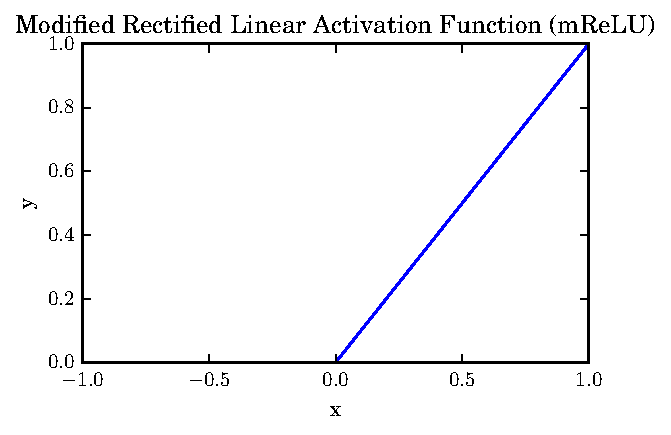
\includegraphics[width=.8\textwidth]{mrelu}
\caption[Modified Rectified Linear Unit Activation]{Modified Rectified Linear Unit Activation Function Plot}
\label{fig:mrelu}
\end{figure}

Since this network is supervised, we allow the training access to the original magnitude spectra $X[k]$. The loss function for training this network is defined as the mean squared error (MSE) between the network output and the clean spectra $X[k]$:

\begin{equation}
l(\vec{X},\vec{\hat{X}}) = \norm{\vec{X}-\vec{\hat{X}}}^{2}
\end{equation}

For our simulations, we also apply batch normalization at the input to help train more quickly and efficiently.

\subsection{Partitioned Autoencoder}

Adopted from \cite{stow}, the partitioned autoencoder is

\subsubsection{Phase Reconstruction}

\subsection{Curro Autoencoder}


